\documentclass{article}

\usepackage[english]{babel}
\usepackage[letterpaper,top=2cm,bottom=2cm,left=3cm,right=3cm,marginparwidth=1.75cm]{geometry}
\usepackage{amsmath}
\usepackage{graphicx}
\usepackage[colorlinks=true, allcolors=blue]{hyperref}
\usepackage{indentfirst}

\title{TPM Key Certification}
\author{Sarah L. Johnson}

\begin{document}
\maketitle

\section*{Relevant Background Definitions}
\subsection*{Key Attributes}
FixedTPM: non-duplicable 

Restricted: operations are limited to TPM-generated data

\subsection*{Key Types}
Primary: Created by TPM based on the current Primary Seed when executing the TPM2\_CreatePrimary command. May be persisted within the TPM. Otherwise must be recreated after a TPM reset.

Ordinary: Created by TPM based on seed taken from the RNG when executing the TPM2\_Create command. Must be the child of another key. May be persisted within the TPM or persisted external to the TPM in the form of an encrypted key blob. The blob is only loadable using the parent key's authorization.

\subsection*{Certificate}
Type: X.509 digital certificate

Public key and data about the subject (i.e., identity) signed by certificate authority

$\text{cert}_{\text{K}} := [(\text{K}, \text{ID})]_{\text{CA}^{-1}}$

Validating a certificate requires a certificate chain in order to verify a chain of trust to a trust anchor (e.g., a root certificate)







\section*{Secure Device Identifier}
\subsection*{Definition}
Identifier that is cryptographically bound to a device

\subsection*{Requirements}
Attestation Key (AK): FixedTPM Restricted signing key

Device Identification Key (DevID): FixedTPM not-Restricted signing key

\subsection*{Initial Keys (IAK/IDevID)}
Created by OEM at manufacturing time

Should be Primary keys

Recommended to be used only for enrollment of an LAK/LDevID

Typically the IAK certificate is the trust anchor for certificates created later

\subsection*{Local Keys (LAK/LDevID)}
Created by owner

Should be Ordinary keys

Recommended to be used only for one application

\subsection*{Note regarding Endorsement Key (EK)}
Cannot be used as a secure device identifier because it is a storage key (not a signing key) and identifies a TPM (not a device)

\section*{Relationships of Keys/Certificates}
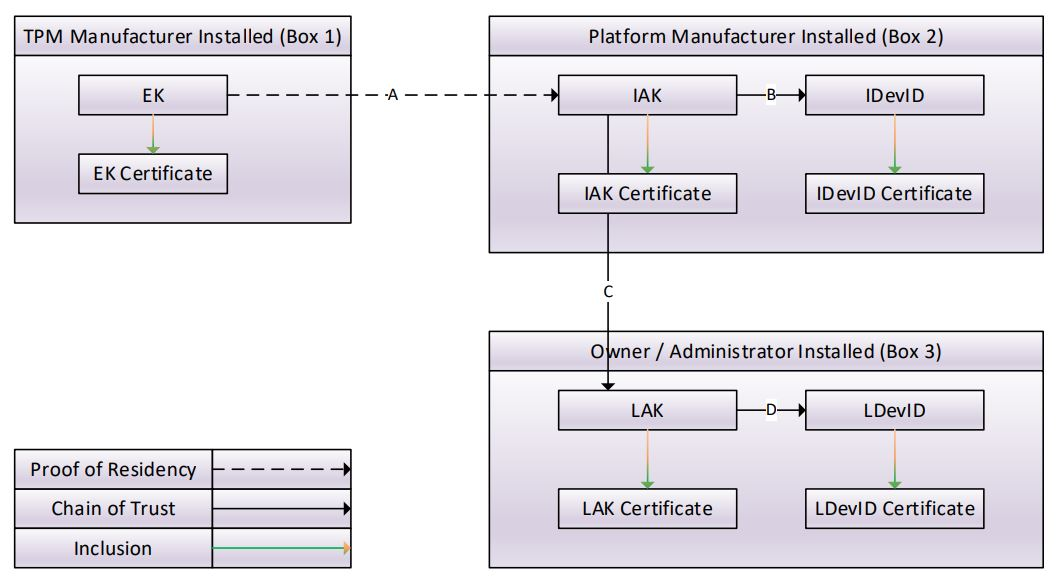
\includegraphics[scale=0.6]{certificateRelationships.jpg}

Box 1: The EK Certificate is signed by the TPM Manufacturer and binds the EK to a specific TPM from that manufacturer

Line A: The IAK is verified by the OEM's CA to have the correct key properties and to be resident in the same TPM as the EK

Line B: The IDevID is verified by the OEM's CA to have the correct key properties and to be resident in the same TPM as the IAK

Box 2: The IAK Certificate and IDevID Certificate is signed by the device OEM's CA and binds the IAK and IDevID to a specific device identity (e.g., model and serial numbers)

Line C: The LAK is verified by the Local CA to have the correct key properties and to be resident in the same TPM as the IAK

Line D: The LDevID is verified by the device owner's CA to have the correct key properties and to be resident in the same TPM as the LAK

Box 3: The LAK Certificate and LDevID Certificate is signed by the device owner's CA

\iffalse
\subsection*{extra}

Prove a new key belongs to a specific device: 1) binding the TPM to the OEM device and 2) binding an AK to a TPM using the EK

An AK certificate is the trust anchor for certificates created later (because it is the certificate that ties a new key to the same TPM containing both keys)

The OEM CA makes an assertion by signing an IAK certificate that is a primary security dependency for later DevID certificate creation

An OEM-supplied IAK certificate is a definitive assertion to applications that need proof that the IAK belongs to a specific device
\fi




\section*{Certificate Authority}
\subsection*{General Requirements}
Must verify TPM residency of a key

Must evaluate TPM data in the certificate signing request

Should support a standard certificate tranport protocol that provides protection from replay attacks and provides confidentiality and integrity (e.g., Enrollment over Secure Transport (EST))


\subsection*{OEM Creation of IAK Certificate based on EK Certificate}

Procedure assures that the new IAK is resident in the same TPM as the EK and that the EK resident in this TPM corresponds to the EK certificate  \\

Detailed Procedure:
\begin{enumerate}
    \item Platform creates the IAK
    \item Platform builds the certificate signing request (i.e., the TCG-CSR-IDEVID structure)
    \begin{enumerate}
        \item Platform identity information (includes the device model and serial number)
        \item The EK certificate
        \item The IAK public area
    \end{enumerate}
    \item Platform uses TPM2\_Hash followed by TPM2\_Sign on the CSR using the new IAK (proves control of the IAK to the CA)
    \item Platform sends the signed CSR to the CA
    \item The CA verifies the received data
    \begin{enumerate}
        \item Verify the signature on the CSR using the IAK public key (extracted from the CSR)
        \item Verify the EK certificate using the TPM manufacturer's public key
        \item Verify the attributes of the IAK
    \end{enumerate}
    \item The CA uses TPM2\_MakeCredential to create an encrypted credential blob 
    \begin{enumerate}
        \item The cryptographic name of the IAK (hash of IAK public area)
        \item Nonce
        \item Encrypted with the EK
    \end{enumerate}
    \item The CA sends the encrypted credential blob to the Platform
    \item The Platform uses TPM2\_ActivateCredential command to release the nonce (proves that the IAK is loaded on the same TPM as the EK)
    \begin{enumerate}
        \item The TPM verifies the IAK's name using the EK
    \end{enumerate}
    \item The Platform returns the nonce to the CA
    \item The CA verifies the nonces match
    \item The CA issues the IAK certificate
\end{enumerate}

\subsection*{Symbolic representation of OEM Creation of IAK Certificate based on EK Certificate}

\begin{enumerate}
    \item TPM2\_Create to get IAK, $\text{IAK}^{-1}$
    \item CSR =
    \begin{enumerate}
        \item deviceInfo = (prodModel, prodSerial)
        \item $\text{cert}_{\text{EK}} = [(\text{EK}, \text{tpmInfo})]_{\text{TPM\_CA}^{-1}}$
        \item IAK
    \end{enumerate}
    \item TPM2\_Hash and TPM2\_Sign to get $[\text{\#CSR}]_{\text{IAK}^{-1}}$
    \item send $[\text{\#CSR}]_{\text{IAK}^{-1}}$
    \item verify $[\text{\#CSR}]_{\text{IAK}^{-1}}$
    \begin{enumerate}
        \item CheckSig $[\text{\#CSR}]_{\text{IAK}^{-1}}$ with IAK
        \item CheckSig $\text{cert}_\text{EK}$ with TPM\_CA
        \item check attributes of IAK
    \end{enumerate}
    \item TPM2\_MakeCredential to get $\{\text{cred}_\text{IAK}\}_\text{EK}$ with $\text{cred}_\text{IAK}$ =
    \begin{enumerate}
        \item \#IAK (name)
        \item r (nonce)
    \end{enumerate}
    \item send $\{\text{cred}_\text{IAK}\}_\text{EK}$
    \item TPM2\_ActivateCredential to get r'
    \begin{enumerate}
        \item Decrypt $\{\text{cred}_\text{IAK}\}_\text{EK}$ with $EK^{-1}$ and check \#IAK
    \end{enumerate}
    \item send r'
    \item check r' = r
    \item send $\text{cert}_{\text{IAK}} = [(\text{IAK}, \text{deviceInfo})]_{\text{OEM\_CA}^{-1}}$
\end{enumerate}

\subsection*{Owner Creation of LAK Certificate based on IAK Certificate}

Procedure assures that the new LAK is resident in the same TPM as the IAK \\

Detailed Procedure:
\begin{enumerate}
    \item Platform creates the LAK
    \item Platform uses TPM2\_Certify command to certify the new LAK with the IAK, producing a signed TPM2B\_Attest structure (proves that the new LAK is on the same TPM as the IAK)
    \item Platform builds the certificate signing request (i.e., the TCG-CSR-LDEVID structure) including:
    \begin{enumerate}
        \item The IAK certificate (identifies device and binds TPM to the device)
        \item The signed TPM2B\_Attest structure (returned by TPM2\_Certify on the LAK)
    \end{enumerate}
    \item Platform uses TPM2\_Hash followed by TPM2\_Sign on the CSR using the new LAK (proves control of the LAK to the CA)
    \item Platform sends the signed CSR to the CA
    \item The CA verifies the received data
    \begin{enumerate}
        \item Verify the signature on the CSR using the LAK public key (extracted from the CSR)
        \item Verify the IAK certificate using the OEM's public key
        \item Verify the signature on the TPM2B\_Attest structure using the IAK public key (extracted from the IAK certificate)
        \item Verify the attributes of the LAK (must be FixedTPM Restricted signing key)
    \end{enumerate}
    \item The CA issues the LAK certificate
\end{enumerate}

\subsection*{Symbolic representation of Owner Creation of LAK Certificate based on IAK Certificate}
\begin{enumerate}
    \item TPM2\_Create to get LAK, $\text{LAK}^{-1}$
    \item TPM2\_Certify to get $[\text{attest}_\text{LAK}]_{\text{IAK}^{-1}}$
    \item CSR =
    \begin{enumerate}
        \item $\text{cert}_\text{IAK} = [(\text{IAK}, \text{deviceInfo})]_{\text{OEM\_CA}^{-1}}$
        \item $[\text{attest}_\text{LAK}]_{\text{IAK}^{-1}}$
        \item LAK
    \end{enumerate}
    \item TPM2\_Hash and TPM2\_Sign to get $[\text{\#CSR}]_{\text{LAK}^{-1}}$
    \item send $[\text{\#CSR}]_{\text{LAK}^{-1}}$
    \item verify $[\text{\#CSR}]_{\text{LAK}^{-1}}$
    \begin{enumerate}
        \item CheckSig $[\text{\#CSR}]_{\text{LAK}^{-1}}$ with LAK
        \item CheckSig $\text{cert}_\text{IAK}$ with OEM\_CA
        \item CheckSig $[\text{attest}_\text{LAK}]_{\text{IAK}^{-1}}$ with IAK
        \item check attributes of LAK
    \end{enumerate}
    \item send $\text{cert}_{\text{LAK}} = [(\text{LAK}, \text{deviceInfo})]_{\text{Local\_CA}^{-1}}$
\end{enumerate}

\end{document}